\begin{framecard}
	{\color{colorbg}
	\bfseries

	\hugetext{Extensive form games\\\& their translation}}
\end{framecard}

\begin{frame}{Extensive form}
	(pic)

	\onslide<2->{
		A \textbf{\textcolor{colornote}{(perfect information)} extensive-form tree} is a term of
		\begin{align*}
			\mbox{data} \;\PETree = \Leaf \;\; {\colar R}^{\colag P}\quad|\quad \Node \;\; \colag P \;\; \colar{(n : \N^+)}\;\; \colar{([n] \to  \PETree)}
		\end{align*}
		where $\colag P$ = set of \textbf{players}, $\colar R$ = type of \textbf{rewards} (usually $\R$).
	}
\end{frame}

\begin{frame}{Extensive form}
	\textbf{\textcolor{coloragents}{Strategies}} can be inductively defined...

	\begin{minipage}[c]{\textwidth}
		\begin{minipage}[c]{.47\textwidth}

		\end{minipage}
		\begin{minipage}[c]{.47\textwidth}
			\begin{align*}
				& \strategies_\PET : \PETree \to P \to \mathsf{Set} \\
				& \strategies_\PET \; (\Leaf \; v)\; p = \One \\
				& \strategies_\PET \; (\Node \; q \; n \; f)\; p\\
				& \qquad = (\mathsf{if}\ p \equiv q\ \mathsf{then}\ [n]\ \mathsf{else}\ \One) \times (\Pi\,{m \in [n]})\, \strategies_\PET\; (f\; m)\; p\\
				&\\
				& \profiles_\PET : \PETree \to \mathsf{Set}\\
				& \profiles_\PET\; T = (\Pi\,p \in P)\ \strategies_\PET\; T\; p
			\end{align*}
		\end{minipage}
	\end{minipage}
\end{frame}

\begin{frame}{Extensive form}
	As well as \textbf{\textcolor{coloragents}{moves}} (= paths in tree) and payoff function:

	\begin{minipage}[c]{\textwidth}
		\begin{minipage}[c]{.47\textwidth}

		\end{minipage}
		\begin{minipage}[c]{.47\textwidth}
			\begin{align*}
				& \paths_\PET : \PETree \to \mathsf{Set} \\
				& \paths_\PET \; (\Leaf \; v) = \One \\
				& \paths_\PET \; (\Node \; p \; n \; f) = (\Sigma\,{m \in [n]}) \; \paths_\PET\; (f\; m)\\
				&\\
				& \payoff_\PET : (T : \PETree) \to (\paths_\PET\;T) \to R^P\\
				& \payoff_\PET \; (\Leaf \; v) \; \unit = v\\
				& \payoff_\PET \; (\Node \; p \; n \; f) \; (m, \pi) = \payoff_\PET\; (f\; m) \; \pi
			\end{align*}
		\end{minipage}
	\end{minipage}
\end{frame}

% \begin{frame}{Extensive form}
% 	A game is presented as a (rooted) tree, which should reflect the possible unfoldings of the game.
% 	Each node is labelled with a \emph{player}. Branches represent possible \emph{moves} and \emph{payoff vectors} await at the leaves.

% 	Two kinds:
% 	\begin{enumerate}
% 		\item Perfect information: any player always knows exactly the state of the game (path from root to their nodes)
% 		\item Imperfect information: otherwise
% 	\end{enumerate}

% 	{\color{colornote}As customary in classical game theory, all players $\argmax$ their payoff.}
% \end{frame}

% \begin{frame}

% \end{frame}

\begin{frame}{Translation}
	Finally, we can translate any $\PETree$ to an open game with agency:

	(pic)

	where
	\begin{enumerate}
		\item $\Dec{[n]}{R^P}$ is the `trivial' game where moves = strategies = $[n]$ and coplay is just $\Delta$.
		\item $\regroup_p$ is regrouping along $\{p\} + P \to P$.
	\end{enumerate}
	and we equip this arena with $\colag{\boxtimes_{p \in P} \argmax (- \cmp \pi_p)}$.
\end{frame}

\begin{frame}{Adding imperfect information}
	Sometimes players can't access the whole state of the game (i.e. history of play)

	\begin{center}
		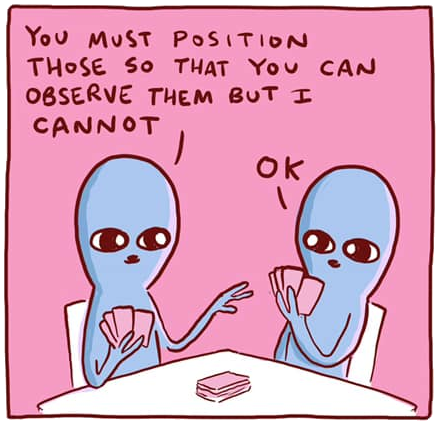
\includegraphics[width=.7\textwidth]{figures/imperfect-information.png}
	\end{center}
\end{frame}

\begin{frame}{Adding imperfect information}
	Information (or better, lack thereof) is represented by sets of 'indistinguishable states' called \textcolor{coloragents}{\textbf{information sets}}
\end{frame}

\begin{frame}{Adding imperfect information}
	\textcolor{coloragents}{Strategies} need to respect information sets: players can't distinguish between states in the same set:

	(pic)

	\textcolor{colornote}{It gets a bit more complicated with mixed strategies.}
\end{frame}


\begin{frame}{Adding imperfect information}
	\begin{definition}
		An \textbf{imperfect information extensive-form tree} is a term of
		\begin{align*}
			\mbox{data} \;\; \IETree = \Leaf \;\; {\colar R}^{\colag P} \ |\  \Node \;\; \colag{(i:I)} \;\; \colar{([n\; i] \to  \IETree)}
		\end{align*}
		where $\colag I : \Set$ is a set of \textbf{information labels} and  $\colar{n : I \to \N^+}$ assigns moves to nodes of the same information set. Additionally, there is an epi map $\colag{\belongs : I \to P}$.
	\end{definition}

	\textbf{Limit case}: all information sets are singletons = perfect information.
\end{frame}


\begin{frame}{Translation}
	\textbf{Idea}: information sets are instances of 'tying' reparametrisations.
	\begin{enumerate}
		\item Forget about information sets and recover a perfect information game:
		\begin{align*}
			& \IETtoPET : \IETree \to \PETree\\
			& \IETtoPET\; (\Leaf\; v) = \Leaf\; v\\
			& \IETtoPET\; (\Node\; i\; f) = \Node\; (\belongs\,i)\; (n\; i)\; (\lambda m \,.\, \IETtoPET\; (f\; m))
		\end{align*}
		\item Translate it using $\PETtoArena$.
		\item Reparametrise along $\colag\clone$ which ties strategies in the same information sets.
	\end{enumerate}
\end{frame}
